\documentclass[conference]{IEEEtran}
%\IEEEoverridecommandlockouts
% The preceding line is only needed to identify funding in the first footnote. If that is unneeded, please comment it out.
\usepackage{cite}
\usepackage{amsmath,amssymb,amsfonts}
\usepackage{algorithmic}
\usepackage{graphicx}
\usepackage{textcomp}
\usepackage{xcolor}
\usepackage{float}
\def\BibTeX{{\rm B\kern-.05em{\sc i\kern-.025em b}\kern-.08em
    T\kern-.1667em\lower.7ex\hbox{E}\kern-.125emX}}
\begin{document}

\title{Exploration of Structural Code Relationship Space for Context Collection Optimization \\
%{\footnotesize \textsuperscript{*}Note: Sub-titles are not captured in Xplore and
%should not be used}
%\thanks{Identify applicable funding agency here. If none, delete this.}
}

\author{\IEEEauthorblockN{Constantinos Sofianos}
\IEEEauthorblockA{\textit{Independent Researcher} \\
Paphos, Cyprus \\ 
costa.sofianos@gmail.com}
}

\maketitle
\begin{abstract}
This paper presents a solution to the Context Collection Competition 
organized by JetBrains and Mustral AI, addressing the challenge of optimizing code completion across diverse 
codebases and multiple LLMs. The application was designed as a dynamic, composable framework, enabling rapid
 experimentation with multiple context-collection strategies. Building on the Kotlin PSI library, a semantic
  tree layer was introduced to capture meaningful code associations and dynamically adjust the level of detail, 
  such as omitting method bodies or private methods. This approach shares similarities with Hierarchical Context Pruning, 
  aiming to maximize the signal-to-noise ratio in retrieved context. 
  While effective with some LLMs—particularly Codestral AI—results varied across models. 
The lack of a scalable test environment limited systematic exploration of strategy parameters. 
Future work will focus on automated large-scale evaluation to fully leverage the framework’s adaptability to 
find upper bounds of performance. 
\end{abstract}

\begin{IEEEkeywords}
code context collection, semantic code analysis, hierarchical context pruning, large language models
\end{IEEEkeywords}

\section{Introduction}
Optimizing code completion using large language models (LLMs) presents significant challenges due to the diversity of 
codebases, the rapid evolution of models, and the complexity of capturing relevant context efficiently. The 
Context Collection Competition, organized by JetBrains and Mistral AI, provided a practical setting to explore
 these challenges, requiring a solution capable of running across multiple Kotlin codebases and three different LLMs 
 under strict performance constraints.

This paper presents a dynamic and composable framework designed to facilitate rapid experimentation
 with multiple context-collection strategies. By extending the Kotlin PSI library with a semantic tree layer, 
 the framework captures meaningful code associations and allows context to be selectively represented—such as 
 omitting method bodies or private methods—to maximize the signal-to-noise ratio. The approach is conceptually 
 similar to Hierarchical Context Pruning \cite{hcp}, focusing on extracting the most relevant context for LLM-based code completion.

Two key lessons emerged during the project. First, the absence of a scalable local test environment 
limited the exploration of parameters and strategies, highlighting the need for automated, 
large-scale evaluation to fully leverage the framework’s adaptability. Second, within the limited experimental 
iterations, certain semantic associations—specifically, identifying references to the classes and methods 
involved—proved more effective than analyzing code that merely referenced the incomplete code. 
These findings highlight promising directions for further refinement.

\section{Design Goals}

\subsection{Framework-Level Goals}
There is no established deterministic method for finding an optimal strategy across diverse codebases and evolving LLMs. 
For this reason, the application was designed to support an experimental approach to context collection. 
To enable effective iteration, the system allows rapid experimentation with different strategies and their 
corresponding parameter tuning, while providing transparency to support a strong feedback loop. 
This transparency ensures that the results of each experiment, including how context snippets are prioritized and selected, 
can be inspected and analyzed to guide further improvements.  In the limited time and resources of the competition project, 
this iterative process was done manually, but the framework is designed to support automated optimisation in future work.

The primary framework-level design goals were thus established as:

\begin{itemize}
    \item \textbf{Composable and Configurable} -- Enable the combination of multiple context collection strategies 
    and built-in ability to experiment with new approaches.
    \item \textbf{Efficiency} -- Adequate performance to support repeated iterations and practical usage.
    \item \textbf{Transparency} -- Makes reasoning behind code selection visible and quantifiable, 
    providing insight into weighting and prioritization to facilitate experimentation and tuning.
\end{itemize}


\subsection{Strategy-Level Goals}
While the framework allowed an unlimited and varied set of strategies, it was important to have a specific focus in 
terms of the types of strategies to be explored.

We defined the choice of strategies as "Strategy-Level Goals" to ensure that the strategies would be aligned with the 
overall objectives of the project.

The strategy-level goals were defined as:
\begin{itemize}
\item \textbf{Precise and Reified Associations} — Code associations have a clear, structured definition and are quantifiable, 
allowing the framework to reason about its significance and influence prioritization and pruning decisions.

\item \textbf{Dynamic} — Support parameterized prioritization and pruning that can adapt to different scenarios, informed by the association data from the previous goal. This flexibility allows experimentation with varying thresholds and 
rules to optimise completion quality for different LLMs and codebases.

\item \textbf{Efficient} — Allow for detection and pruning with minimal computational overhead, 
ensuring that the strategy operates within acceptable performance constraints while maintaining the 
precision and adaptability established in the other goals.
\end{itemize}



\section{Solution and Implementation}

\subsection{Strategy Combination Executor}
Each strategy runs independently and produces its own set of code context entries. The entries are then 
combined by the Context Collector to provide the final context for the LLM.  After prioritisation, the Context Collector
limits the entries inserted into the final context to be within bounds of the LLM being used. In addition,
in order to meet the design goal of transparency, a report is created which displays the entries with their 
associated weights along with how they were derived. Figure~\ref{fig:strategy-combining} 
shows an overview of this design.


\begin{figure}[htbp]
\centerline{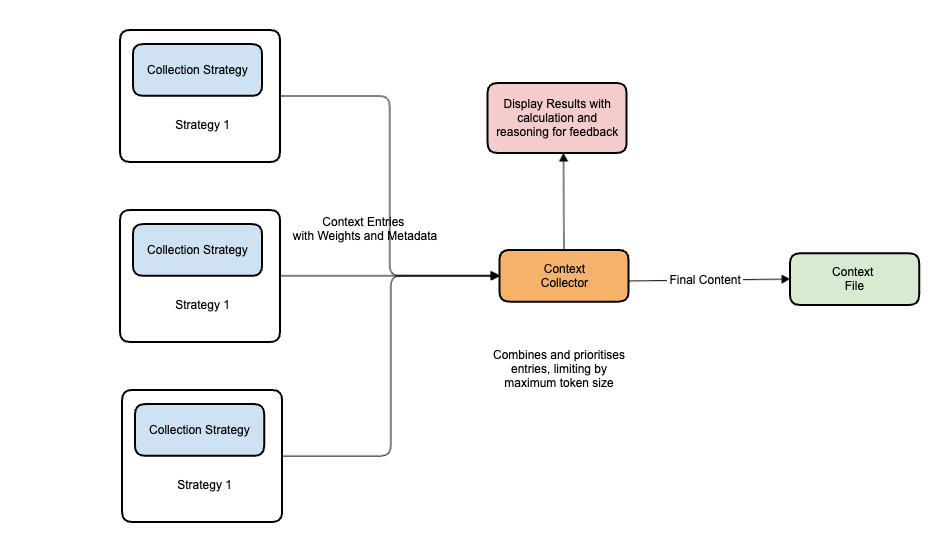
\includegraphics[width=0.5\textwidth]{StrategyCombiningArchitecture.png}}
\caption{Architecture used for Strategy Composition and Reporting.}
\label{fig:strategy-combining}
\end{figure}

\subsection{Dynamic Computation Caching}
To meet the goals of efficiency and experimental strategy support, 
an automated caching layer was introduced to compute and store results for reuse. 
Computations, such as indexing references or creating a parsed semantic tree, are automatically generated when requested by a strategy. 
On-demand creation accommodates chains of dependencies: for example, if a strategy requires a semantic tree, 
and the semantic tree requires a PSI tree, the system automatically creates and caches both for reuse by other strategies. 
This approach enables experimentation with different strategy combinations without incurring redundant computation. 
Figure~\ref{fig:computation-cache} illustrates the architecture.


\begin{figure}[htbp]
\centerline{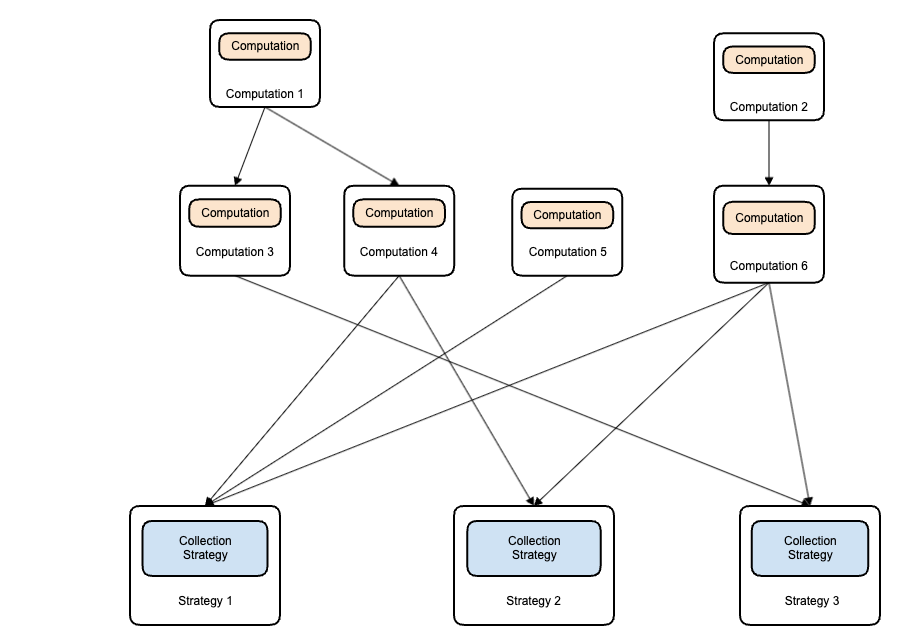
\includegraphics[width=0.5\textwidth]{CachedComputationArchitecture.png}}
\caption{Architecture of the computation caching system.}
\label{fig:computation-cache}
\end{figure}

\subsection{Result Reporting} 
The results of each strategy are returned in a result object structure that contains the code snippets, 
their weights, and the reasoning behind their selection.  This structure is then used to create an HTML report that
displays the results in a human-readable format.  As discussed in the design goals section, this report is essential for
the experimental nature of the framework, as it allows for easy inspection and analysis of the results.

\subsection{Psi Tree and Semantic Tree Parser}
Given the limited time and resources of the competition project, a decision was made to focus on a single language and approach the problem in a focused direction.  Kotlin 
was chosen as the language, and the focus was on using the code structure to inform the context collection strategies. 

Initially, the Kotlin PSI library was used to parse the code and create a PSI tree. 
This provided a basic way to identify relationships among code elements, but its limitations 
became apparent for more complex relationships. 
The PSI tree represents the code syntactically and does not capture semantic relationships, 
which are often more relevant for code completion. While it works for simple name matching, 
it does not differentiate between classes, methods, or variables, which must be inferred by traversing the tree and applying rules. 
For example, a KtNamedReference does not indicate whether the element is a class, method, or variable. 
Additionally, the PSI tree does not resolve references directly.
Although methods like the Binding Context exist for this purpose, they are resource intensive and do not meet efficiency requirements.

To balance the design goals within limited time and resources, a hierarchical representation of the source code was created, 
called the Semantic Tree. Built on top of the PSI tree, it captures key language elements—classes, methods, and variables—and their 
compositional relationships.

The basic outline of the hierarchy is shown in Figure~\ref{fig:semantic-tree}.

The Semantic Tree provides a way to traverse the code structure in a direct and efficient way that is not 
possible with the Psi Tree.  Each node in the hierarchy is linked to the originating Psi Element, which means that there is a 
link to the original syntactic tree and the related source code.

Linking nodes to the original code enables dynamic creation of snippets by selecting which elements to include. 
For example, a node's association weight can determine whether to include the full method body or just the method signature. 
This dynamic adjustment of detail is a key strategy in the HCP approach \cite{hcp}.


\begin{figure}[htbp]
\centerline{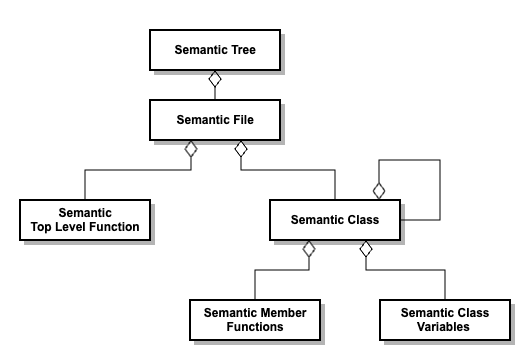
\includegraphics[width=0.5\textwidth]{SemanticPsiTreeNodeHierarchy.png}}
\caption{Hierarchy of nodes in the Semantic Tree built on top of the Psi Tree. This simple abstraction of the code structure
allows for efficient traversal and association of code elements.}
\label{fig:semantic-tree}
\end{figure}

 
\section{Experiments and Evaluation}

With the framework in place, there were multiple options for experimentation and evaluation. 
Each iteration in the experimentation process was defined by a set of parameters, 
where a parameter represents a chosen value along one of several dimensions.
These parameters controlled both selection of code and its prioritization or pruning—that is, 
not only what code to include in the context, but also how to include it. 
An association was defined between the node in the edit location and a node in the codebase.  
The configuration space was explored along the following dimensions:
\begin{itemize}
\item \textbf{Public or Private Access} Is the associated code accessible from the edit location?
\item \textbf{Reference Direction} Is the associated node referenced by the edit location, or does it reference a node in the edit location?
\item \textbf{Shared References} Does this node share the same references with the edit location?
\item \textbf{Method Matching} Does an associated method match the name of a method in the edit location?
\item \textbf{Proximity to Edit Location} Is the association from code in close proximity to the edit location. 
\item \textbf{Modified Code} Does the associated code belong to a file that has been modified in the current commit?
\item \textbf{Max Token Size} How much code should be included in the context?
\end{itemize}

A manual experimentation process was followed by adjusting these parameters and their impact on the collected context. 
Impact in this context means not only whether to include a some context, but also which parts of the code to include.

Example approaches included:
\begin{itemize}
    \item Show method signatures and include method bodies only when certain parameters are met.  This could be any parameter such as whether the code has been recently modified or whether it is close to the edit location.
    \item Only include code which is referenced from the edit location, and do not include code which uses the edited class or method.
    \item Sort collected context on weight and exclude lower weighted code until the context fits within the token limit.
       
\end{itemize}

The configuration space of all the parameters was traversed manually using feedback of each iteration to move toward an optimum. 
The results of each experiment were easily inspected and analyzed to determine the direction of subsequent iterations. 


As can be readily observed, the space of possible configurations is very large.
 The differing effects of configurations on various LLMs further increased the number of possible permutations in 
 the experimentation process. A representative sample of experiments, illustrating the progression toward the best average score across all
  models, is shown in Table~\ref{tab:results}. The table clearly indicates that the exploration 
of the configuration space did not establish the upper bounds of performance, either for the average score or for the individual models.


\begin{table}[htbp]
\caption{Sample of Parameter Traversal with Results}
\centering
\begin{tabular}{|p{3.5cm}|c|c|c|c|}
\hline
\textbf{Parameter Change} & \textbf{Mellum} & \textbf{Codestral} & \textbf{Qwen} & \textbf{Average}  \\
\hline
Included full files & 0.6227 & 0.6560 & 0.6057 & 0.6282  \\
\hline
Pruned context & 0.6155 & 0.7111 & 0.5957 & 0.6408  \\
\hline
Selective Pruning & 0.6468 & 0.6921 & 0.5924 & 0.6438  \\
\hline
Include Incoming References & 0.6668 & 0.6897 & 0.6016 & 0.6527  \\
\hline
Remove Incoming References& 0.6879 & 0.7372 & 0.5729 & 0.6660  \\
\hline
Added matching methods & 0.6808 & 0.7308 & 0.6300 & 0.6710  \\
\hline
\end{tabular}
\label{tab:results}
\end{table}



\section{Results and Findings}

The experimentation results yielded several important findings, summarized below.

Key Findings:
\begin{itemize}
\item \textbf{Model Performance Differences} — Codestral consistently outperformed the other LLMs across most configurations, followed by Mellum and Qwen-Coder.
\item \textbf{Hierarchical Context Pruning} — Removing method bodies and inaccessible code improved performance for all LLMs in nearly all cases.
\item \textbf{Association Direction} — Code referenced \emph{from} the edit location positively influenced performance, whereas code that referenced \emph{to} the edit location often reduced it.
\item \textbf{Recency of Modifications} — Prioritizing recently modified code consistently improved performance.
\item \textbf{Name Matching Sensitivity} — Providing implementations of methods with names similar to the edited method generally improved performance, but was highly sensitive to the number of matches, method body size, and other parameters.
\end{itemize}

Summary.
These findings demonstrate clear performance differences across LLMs and identify configurations that consistently improve results. They also reveal trade-offs—such as when full context or 
excessive name-matching reduces performance—that help delineate the 
conditions under which the approach is most effective.

\section{Discussion and Future Work}

The results suggest that concise structural associations, particularly method signatures of elements referenced from the edit location, 
carry the most useful signal for code completion. Providing full code details, such as entire files or method bodies, benefited some models, 
such as Codestral, but the advantage was not universal and requires precise tuning per model. 
Codestral consistently outperformed the other LLMs across various configurations,
 indicating strong compatibility with the overall strategy. Mellum showed moderate performance, 
 while Qwen-Coder performed significantly worse. The reasons for Qwen-Coder’s lower performance are not yet clear and warrant 
 further investigation.

Parameter adjustments were made iteratively using feedback to manually traverse the configuration space in search of optimal performance.  
Limitations of the local test environment required that tests be conducted online, which constrained the number of submissions.  
This manual approach, combined with the large number of possible permutations, 
means that the configuration space was not exhaustively explored, either for individual LLMs or for the overall score.

Parameter settings often had opposite effects across different LLMs, suggesting that 
each model may require tailored optimization. A more comprehensive exploration of the parameter space for 
each LLM could provide clearer insights into their individual strengths and reveal the potential performance 
achievable with this approach. Such exploration may reveal configurations where lower-performing models, 
such as Qwen-Coder, achieve improved results.

Based on these observations, a clear direction for future work is evident. Establishing a scalable local test environment, 
combined with extending the framework to programmatically explore the parameter space for each LLM independently,
 would enable more systematic experimentation. The existing framework design supports such an extension. 
 Additionally, the framework can be extended to incorporate other successful strategies, allowing the discovery 
 of optimal combinations and further improvements in performance.
\section{Conclusion}

This paper presents a framework for selecting and pruning code context to optimize LLM-assisted code completion.
It is shown that concise structural associations, particularly method signatures of elements referenced from the edit location, provide the most useful signals, and that pruning of irrelevant code consistently improves performance across models.
The framework’s adaptability allows experimentation with different context selection strategies and parameter settings.
Applying a strategy that selects and prunes code context based on semantic associations demonstrates the effectiveness 
of this approach for LLM-assisted code completion.

Overall, it is demonstrated that leveraging semantic structure and targeted pruning is an effective strategy for 
code context selection, providing a foundation for more efficient and model-aware code completion.

The results also demonstrate that model performance varies significantly with configuration choices, 
indicating that programmatic exploration of the configuration space can identify optimal settings for 
individual LLMs or across multiple models. Such optimization, including combining additional context selection strategies 
with semantic-pruning approaches, 
can help fine-tune performance and approach the upper bounds of achievable results.


\begin{thebibliography}{00}
\bibitem{hcp} L. Zhang, Y. Li, J. Li, X. Xia, J. Yang, R. Luo, M. Wang, L. Chen, J. Liu, and M. Yang, ``Hierarchical Context Pruning: Optimizing Real-World Code Completion with Repository-Level Pretrained Code LLMs,'' arXiv preprint arXiv:2406.18294, 2024. [Online]. Available: https://arxiv.org/abs/2406.18294
\end{thebibliography}
\vspace{12pt}
\end{document}
